%% LyX 1.3 created this file.  For more info, see http://www.lyx.org/.
%% Do not edit unless you really know what you are doing.
\documentclass[english, 12pt]{article}
\usepackage{times}
%\usepackage{algorithm2e}
\usepackage{url}
\usepackage{bbm}
\usepackage[T1]{fontenc}
\usepackage[latin1]{inputenc}
\usepackage{geometry}
\geometry{verbose,letterpaper,tmargin=2cm,bmargin=2cm,lmargin=1.5cm,rmargin=1.5cm}
\usepackage{rotating}
\usepackage{color}
\usepackage{graphicx}
\usepackage{subcaption}
\usepackage{amsmath, amsthm, amssymb}
\usepackage{setspace}
\usepackage{lineno}
\usepackage{hyperref}
\usepackage{bbm}
\usepackage{makecell}

\renewcommand{\arraystretch}{1.2}

%\usepackage{xr}
%\externaldocument{SCT-supp}

%\linenumbers
%\doublespacing
\onehalfspacing
%\usepackage[authoryear]{natbib}
\usepackage{natbib} \bibpunct{(}{)}{;}{author-year}{}{,}

%Pour les rajouts
\usepackage{color}
\definecolor{trustcolor}{rgb}{0,0,1}

\usepackage{dsfont}
\usepackage[warn]{textcomp}
\usepackage{adjustbox}
\usepackage{multirow}
\usepackage{graphicx}
\graphicspath{{../figures/}}
\DeclareMathOperator*{\argmin}{\arg\!\min}

\let\tabbeg\tabular
\let\tabend\endtabular
\renewenvironment{tabular}{\begin{adjustbox}{max width=0.9\textwidth}\tabbeg}{\tabend\end{adjustbox}}

\makeatletter

%%%%%%%%%%%%%%%%%%%%%%%%%%%%%% LyX specific LaTeX commands.
%% Bold symbol macro for standard LaTeX users
%\newcommand{\boldsymbol}[1]{\mbox{\boldmath $#1$}}

%% Because html converters don't know tabularnewline
\providecommand{\tabularnewline}{\\}

\usepackage{babel}
\makeatother


\begin{document}


\title{Insights on ancestry using principal component analysis of genetic data}
\author{Florian Priv\'e$^{\text{1,}*}$ and Bjarni J. Vilhj\'almsson$^{\text{1}}$}

\date{~ }
\maketitle

\noindent$^{\text{\sf 1}}$National Centre for Register-Based Research, Aarhus University, Aarhus, 8210, Denmark. \\
\noindent$^\ast$To whom correspondence should be addressed.\\

\noindent Contact:
\begin{itemize}
\item \url{florian.prive.21@gmail.com}
\end{itemize}

\newpage

\abstract{
}


%%%%%%%%%%%%%%%%%%%%%%%%%%%%%%%%%%%%%%%%%%%%%%%%%%%%%%%%%%%%%%%%%%%%%%%%%%%%%%%%

\newpage

\section{Introduction}

%%%%%%%%%%%%%%%%%%%%%%%%%%%%%%%%%%%%%%%%%%%%%%%%%%%%%%%%%%%%%%%%%%%%%%%%%%%%%%%%

\section{Material and Methods}

\subsection{Ancestry matching \label{ancestry}}

We use the 1000 Genomes (1000G) Project data \cite[]{10002015global} to infer the ancestry of individuals from a study dataset using the following steps: 1) we project individuals from the study dataset onto the PCA space computed using the 1000G data \cite[]{prive2020efficient}; 2) we compute the robust center and covariance parameters of the Mahalanobis distance \cite[]{prive2020efficient} for each of the 26 populations of the 1000G data; 3) we compute the Mahalanobis distance for each projected individual of the study data and each population of the 1000G data (using the center and covariance parameters computed previously); 4) we derive p-values from those distances, as they are approximately chi-squared distributed with the number of PCs used for computing the distances as degrees of freedom; 5) we affect each individual to the largest corresponding p-value (smallest distance), but discard individuals whose maximum p-value is less than 0.05 (i.e.\ individuals far from every population of the 1000G data). 

\subsection{Distance between two populations}

To infer a PCA-based genetic distance between two populations, we use the Bhattacharyya distance between two multivariate normal distributions $\mathcal{N}(\boldsymbol\mu_1,\,\boldsymbol\Sigma_1)$ and $\mathcal{N}(\boldsymbol\mu_2,\,\boldsymbol\Sigma_2)$ as defined as
$$D_B={1\over 8}(\boldsymbol\mu_2-\boldsymbol\mu_1)^T \boldsymbol\Sigma^{-1}(\boldsymbol\mu_2-\boldsymbol\mu_1)+{1\over 2}\log \,\left({|\boldsymbol\Sigma| \over \sqrt{|\boldsymbol\Sigma_1| \, |\boldsymbol\Sigma_2|} }\right)~,$$
where $\boldsymbol\Sigma={\boldsymbol\Sigma_1+\boldsymbol\Sigma_2 \over 2}$ and $|M|$ is the absolute value of the determinant of matrix $M$ \cite[]{bhattacharyya1943measure,fukunaga1990introduction}. 
The mean and covariance parameters for each population are computed using the robust center and covariance parameters as in section \ref{ancestry}.

%%%%%%%%%%%%%%%%%%%%%%%%%%%%%%%%%%%%%%%%%%%%%%%%%%%%%%%%%%%%%%%%%%%%%%%%%%%%%%%%

\section{Results}


\subsection{Ancestry matching}

We performed ancestry estimation of the individuals in the UK Biobank using the 1000G data (Section \ref{ancestry}), discarding individuals with unknown ancestry or mixed ancestry.
We did not infer ancestry for 15.9\% of UK Biobank that had a maximum p-value smaller than 0.05 (Figure \ref{fig:ancestry-pval}). 
More precisely, among ``White'', ``British'' and ``Irish'' ancestries, this represented respectively 20.2\%, 11.1\% and 20.3\%, while this represented between 44.5\% (``Chinese'') and 74.3\% (``Bangladeshi'') for other populations. 
In other words, 3 out of 4 of the UK Biobank individual who self-reports as ``Bangladeshi'' could not be attributed to any 1000G population, although 1000G data includes several ``Bengali in Bangladesh'' (SAS\_BEB).
Only 10 people out of 401,048 were wrongly classified in ``super'' population of the 1000G; e.g.\ one Chinese person was classified as European by our method (Table \ref{tab:ancestry-pred}). 
Moreover, our method is able to accurately differentiate between sub-continental populations such as differentiating between Pakistani, Bangladeshi and Chinese people (Table \ref{tab:ancestry-pred}).

% latex table generated in R 3.6.0 by xtable 1.8-4 package
% Mon Oct 21 15:14:34 2019
\begin{table}[ht]
\centering
\caption{Self-reported ancestry (top) of UKBB individuals and their matching to 1000G populations (left) by our method. See the description of 1000G populations at \url{https://www.internationalgenome.org/category/population/}.} 
\label{tab:ancestry-pred}
\begin{tabular}{|l|c|c|c|c|c|c|c|c|c|c|c|c|c|}
  \hline
 & British & Irish & White & Other White & Indian & Pakistani & Bangladeshi & Chinese & Other Asian & Caribbean & African & Other Black & NA \\ 
  \hline
AFR\_ACB &  &  &  &  &  &  &  &  &  & 1832 & 580 & 31 & 259 \\ 
  AFR\_ASW &  &  &  &  &  &  &  &  &  & 315 & 13 & 10 & 39 \\ 
  AFR\_ESN &  &  &  &  &  &  &  &  &  &  & 155 & 1 & 29 \\ 
  AFR\_GWD &  &  &  &  &  &  &  &  &  &  & 20 &  & 4 \\ 
  AFR\_LWK &  &  &  &  &  &  &  &  &  &  & 34 &  & 4 \\ 
  AFR\_MSL &  &  &  &  &  &  &  &  &  &  & 26 &  &  \\ 
  AFR\_YRI &  &  &  &  &  &  &  &  &  & 5 & 469 & 3 & 81 \\ 
   \hline
AMR\_CLM & 1 &  &  & 50 &  &  &  &  &  &  &  &  & 142 \\ 
  AMR\_MXL &  &  & 1 & 3 &  &  &  &  &  &  &  &  & 20 \\ 
  AMR\_PEL &  &  &  & 2 &  &  &  &  &  &  &  &  & 19 \\ 
   \hline
EAS\_CDX &  &  &  &  &  &  &  & 2 &  &  &  &  & 1 \\ 
  EAS\_CHB & 1 &  &  &  &  &  &  & 445 & 10 &  &  &  & 7 \\ 
  EAS\_CHS &  &  &  &  &  &  &  & 380 & 9 &  &  &  & 21 \\ 
  EAS\_JPT &  &  &  &  &  &  &  & 3 & 25 &  &  &  & 122 \\ 
  EAS\_KHV &  &  &  &  &  &  &  & 4 & 16 &  &  &  & 22 \\ 
   \hline
EUR\_CEU & 325725 & 6675 & 350 & 4855 &  &  &  & 1 &  &  &  &  & 1363 \\ 
  EUR\_FIN & 2 &  &  & 118 &  &  &  &  &  &  &  &  & 1 \\ 
  EUR\_GBR & 57497 & 3486 & 79 & 454 &  &  &  &  &  &  & 1 &  & 244 \\ 
  EUR\_IBS & 28 &  & 4 & 452 &  &  &  &  &  &  &  &  & 8 \\ 
  EUR\_TSI & 25 &  & 1 & 177 &  &  &  &  &  &  &  &  & 5 \\ 
   \hline
SAS\_BEB &  &  &  &  & 11 &  & 57 &  &  &  &  &  & 7 \\ 
  SAS\_GIH &  &  &  &  & 334 &  &  &  & 1 &  &  &  & 4 \\ 
  SAS\_ITU & 1 &  &  &  & 314 & 1 &  &  & 264 & 3 &  &  & 82 \\ 
  SAS\_PJL & 1 &  &  &  & 1749 & 767 &  &  & 104 & 2 &  &  & 177 \\ 
  SAS\_STU &  &  &  &  & 38 &  &  &  & 185 &  &  &  & 40 \\ 
   \hline
NA & 47748 & 2594 & 110 & 9705 & 3270 & 980 & 164 & 669 & 1133 & 2140 & 1906 & 73 & 6970 \\ 
   \hline
\end{tabular}
\end{table}

\noindent[OKAY TO CLASSIFY SOME OTHER WHITE AS CENTRAL/SOUTH AMERICANS? MAYBE, SEE NEXT SUBSECTION]

We also  applied our ancestry detection technique to projected individuals from other datasets.
When applied to the European individuals of the POPRES data \cite[]{nelson2008population}, we show that 56.5\% of individuals could not be matched to one of the 26 populations of the 1000G data (Table \ref{tab:ancestry-pred-popres}). 
This is particularly dramatic for all East-Europeans, whose only 11 people could be matched out of 179 (6.1\%).
Moreover, even though 1000G data include several ``Toscani in Italia'' (EUR\_TSI), we were able to match 14.2\% of Italians only.
Nevertheless, all individuals that we could match were identified as of European ancestry. We could also identify accurately sub-regions of Europe; e.g.\ all Spanish and Portugese individuals that we could match (73.1\%) were identified as ``Iberian Population in Spain'' (EUR\_IBS, Table \ref{tab:ancestry-pred-popres}).
Finally, we also projected and matched people from a case-control cohort for celiac disease composed of four European countries: Italy, the Netherlands, the UK and Finland \cite[]{dubois2010multiple}. 
Among UK individuals, 5397 (79.9\%) were matched to either ``Utah Residents with Northern and Western European Ancestry'' (EUR\_CEU) or ``British in England and Scotland'' (EUR\_GBR), 10 (0.2\%) to other European populations, 1 to ``Mexican Ancestry from Los Angeles USA'' (AMR\_MXL) and 1346 (19.9\%) could not be matched (Table \ref{tab:ancestry-pred-celiac}).
Among Finns, 1543 (62.4\%) were matched to ``Finnish in Finland'' (EUR\_FIN), 6 (0.3\%) to other European populations, and 922 (37.3\%) could not be matched.
Among Italians, 229 (22\%) were matched to EUR\_TSI, 15 (1.5\%) to EUR\_IBS and 795 (76.5\%) could not be matched (Table \ref{tab:ancestry-pred-celiac}).

\noindent[USE FIG S1 TO JUSTIFY 5\% THRESHOLD?]

\subsection{Distance between 1000G populations}

\begin{figure}[!htpb]
	\centerline{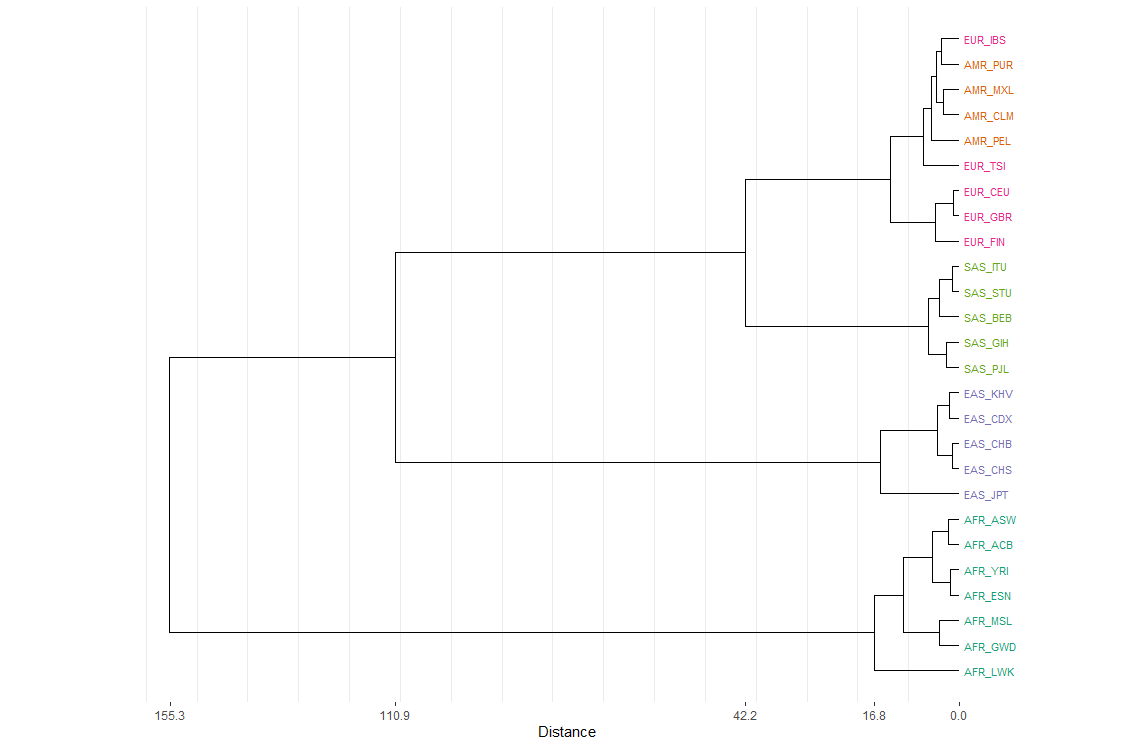
\includegraphics[width=0.9\textwidth]{hclust-pop-1000G.png}}
	\caption{Dendrogram of PC-based distances between populations of the 1000G data. See the description of 1000G populations at \url{https://www.internationalgenome.org/category/population/}. \label{fig:ancestry-dist}}
\end{figure}

\noindent[WHAT TO SAY ABOUT THIS? DISTANCE INFORMATIVE? SAS CLOSER TO EUR THAN EAS?]


\noindent[DO THIS IN OTHER DATASETS? COULD SHOW THAT EAST EUROPEAN FAR FROM 1000G POPS IN POPRES. WHAT ABOUT UKBB?]

%%%%%%%%%%%%%%%%%%%%%%%%%%%%%%%%%%%%%%%%%%%%%%%%%%%%%%%%%%%%%%%%%%%%%%%%%%%%%%%%

\section{Discussion}

\noindent[DISCUSS LACK OF CERTAIN POPULATIONS IN 1000G]

\noindent[DISCUSS PC-BASED GENETIC DISTANCES BETWEEN POPULATIONS]

\noindent[IMPLICATIONS FOR PRS?]




%%%%%%%%%%%%%%%%%%%%%%%%%%%%%%%%%%%%%%%%%%%%%%%%%%%%%%%%%%%%%%%%%%%%%%%%%%%%%%%%


\clearpage

\section*{Software and code availability}

%R package pcadapt is available on CRAN.
%A tutorial on using pcadapt to detect local adaptation is available at \url{https://bcm-uga.github.io/pcadapt/articles/pcadapt.html}.
%The code used in this paper is available at \url{https://github.com/bcm-uga/pcadapt/tree/master/new-paper/code}.

\section*{Acknowledgements}

F.P.\ and B.V.\ are supported by the Danish National Research Foundation (Niels Bohr Professorship to John McGrath).

\section*{Declaration of Interests}

The authors declare no competing interests.

%%%%%%%%%%%%%%%%%%%%%%%%%%%%%%%%%%%%%%%%%%%%%%%%%%%%%%%%%%%%%%%%%%%%%%%%%%%%%%%%

%\newpage

\bibliographystyle{natbib}
\bibliography{refs}

%%%%%%%%%%%%%%%%%%%%%%%%%%%%%%%%%%%%%%%%%%%%%%%%%%%%%%%%%%%%%%%%%%%%%%%%%%%%%%%%

\newpage
\section*{Supplementary Materials}

\renewcommand{\thefigure}{S\arabic{figure}}
\setcounter{figure}{0}
\renewcommand{\thetable}{S\arabic{table}}
\setcounter{table}{0}

%%%%%%%%%%%%%%%%%%%%%%%%%%%%%%%%%%%%%%%%%%%%%%%%%%%%%%%%%%%%%%%%%%%%%%%%%%%%%%%%

%\clearpage

%\subsection*{Supplementary figures}


%%%%%%%%%%%%%%%%%%%%%%%%%%%%%%%%%%%%%%%%%%%%%%%%%%%%%%%%%%%%%%%%%%%%%%%%%%%%%%%%

%\vspace*{1em}

\begin{figure}[!htpb]
\centerline{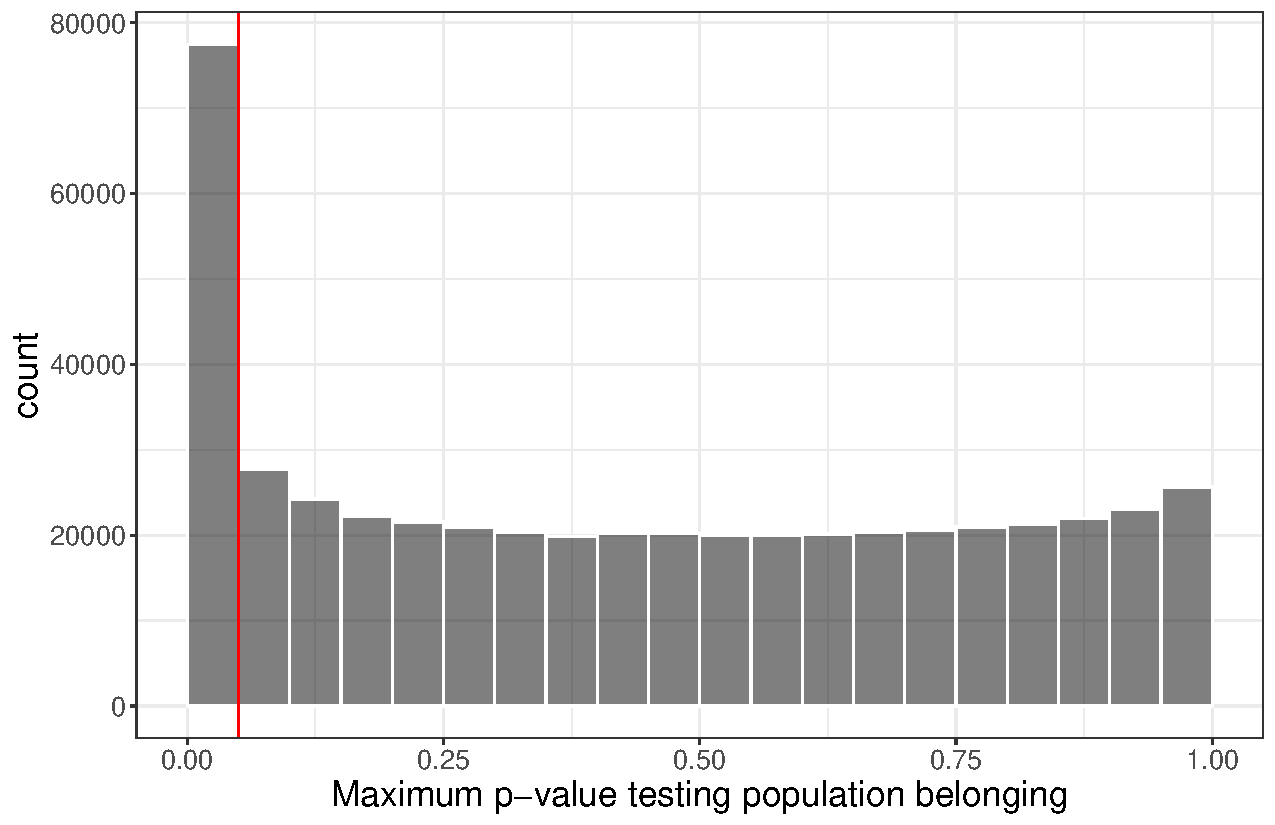
\includegraphics[width=0.8\textwidth]{hist-pval-max.pdf}}
\caption{Maximum p-values based on robust Mahalabonis distances of UK Biobank individuals from each of the 26 1000G populations.
\label{fig:ancestry-pval}}
\end{figure}

%%%%%%%%%%%%%%%%%%%%%%%%%%%%%%%%%%%%%%%%%%%%%%%%%%%%%%%%%%%%%%%%%%%%%%%%%%%%%%%%

% latex table generated in R 3.6.0 by xtable 1.8-4 package
% Sat Oct 19 00:18:24 2019
\begin{table}[ht]
\centering
\caption{Ancestry (left) of POPRES individuals and their matching to 1000G populations (top) by our method. See the description of 1000G populations at \url{https://www.internationalgenome.org/category/population/}.} 
\label{tab:ancestry-pred-popres}
\begin{tabular}{|l|c|c|c|c|c|}
  \hline
 & EUR\_CEU & EUR\_GBR & EUR\_IBS & EUR\_TSI & NA \\ 
  \hline
Anglo-Irish Isles & 159 & 57 &  &  & 50 \\ 
  Belgium & 28 & 3 &  &  & 12 \\ 
  Central Europe & 3 &  &  & 1 & 51 \\ 
  Eastern Europe & 2 &  &  &  & 28 \\ 
  France & 14 &  & 13 &  & 62 \\ 
  Germany & 37 &  &  &  & 34 \\ 
  Italy &  &  & 12 & 19 & 188 \\ 
  Netherlands & 10 & 2 &  &  & 5 \\ 
  Scandinavia & 5 &  &  &  & 10 \\ 
  SE Europe &  &  &  & 5 & 89 \\ 
  SW Europe &  &  & 193 &  & 71 \\ 
  Switzerland & 33 & 1 & 6 &  & 182 \\ 
   \hline
\end{tabular}
\end{table}

% latex table generated in R 3.6.0 by xtable 1.8-4 package
% Sat Oct 19 00:28:24 2019
\begin{table}[ht]
\centering
\caption{Ancestry (left) of Celiac individuals and their matching to 1000G populations (top) by our method. See the description of 1000G populations at \url{https://www.internationalgenome.org/category/population/}.} 
\label{tab:ancestry-pred-celiac}
\begin{tabular}{|l|c|c|c|c|c|c|c|}
  \hline
 & AMR\_MXL & EUR\_CEU & EUR\_FIN & EUR\_GBR & EUR\_IBS & EUR\_TSI & NA \\ 
  \hline
Finland &  & 4 & 1543 & 1 &  & 1 & 922 \\ 
  Italy &  &  &  &  & 15 & 229 & 795 \\ 
  Netherlands &  & 802 &  & 382 & 1 &  & 463 \\ 
  UK & 1 & 2865 & 1 & 2532 & 4 & 5 & 1346 \\ 
   \hline
\end{tabular}
\end{table}


\end{document}
